\documentclass[8pt]{extarticle}
\title{}
\author{Avinash Iyer}
\date{}
\usepackage[shortlabels]{enumitem}

%font setup
%
%\usepackage{newpxtext,eulerpx}

%paper setup
\usepackage{geometry}
\geometry{letterpaper, portrait, margin=1in}
\usepackage{fancyhdr}

%symbols
\usepackage{amsmath}
\usepackage{amssymb}
\usepackage{mathtools}
\usepackage{hyperref}
\usepackage{gensymb}

\usepackage[T1]{fontenc}
\usepackage[utf8]{inputenc}

%chemistry stuff
\usepackage[version=4]{mhchem}
\usepackage{chemfig}

%plotting
\usepackage{pgfplots}
\usepackage{tikz}
\tikzset{middleweight/.style={pos = 0.5, fill=white}}
\tikzset{weight/.style={pos = 0.5, fill = white}}
\tikzset{lateweight/.style={pos = 0.75, fill = white}}
\tikzset{earlyweight/.style={pos = 0.25, fill=white}}

%\usepackage{natbib}

%graphics stuff
\usepackage{graphicx}
\usepackage{svg}
\graphicspath{ {./images/} }

%code stuff
%when using minted, make sure to add the -shell-escape flag
%you can use lstlisting if you don't want to use minted
%\usepackage{minted}
%\usemintedstyle{pastie}
%\newminted[javacode]{java}{frame=lines,framesep=2mm,linenos=true,fontsize=\footnotesize,tabsize=3,autogobble,}
%\newminted[cppcode]{cpp}{frame=lines,framesep=2mm,linenos=true,fontsize=\footnotesize,tabsize=3,autogobble,}

\usepackage{listings}
\usepackage{color}
\definecolor{dkgreen}{rgb}{0,0.6,0}
\definecolor{gray}{rgb}{0.5,0.5,0.5}
\definecolor{mauve}{rgb}{0.58,0,0.82}

\lstset{frame=tb,
	language=Java,
	aboveskip=3mm,
	belowskip=3mm,
	showstringspaces=false,
	columns=flexible,
	basicstyle={\small\ttfamily},
	numbers=none,
	numberstyle=\tiny\color{gray},
	keywordstyle=\color{blue},
	commentstyle=\color{dkgreen},
	stringstyle=\color{mauve},
	breaklines=true,
	breakatwhitespace=true,
	tabsize=3
}
% text + color boxes
\usepackage[most]{tcolorbox}
\tcbuselibrary{breakable}
\newtcolorbox{problem}[1]{colback = white, title = {#1}, breakable}
\newtcolorbox{solution}{colback = white, colframe = black!75!white, title = Solution, breakable}
%including PDFs
\usepackage{pdfpages}
\setlength{\parindent}{0pt}

\pagestyle{fancy}
\fancyhf{}
\rhead{Avinash Iyer}
\lhead{Math 212: Class Notes}
\begin{document}
  \begin{problem}{The basis of Multivariable Calculus}
    If a function is continuous and differentiable, on a small enough interval, the function will approximate a line (i.e., a function of $x$).\\

    A similar intuition applies to functions of more than one variable (but with a plane, cube, hypercube, etc.). However, in multivariable functions, we will have to sacrifice the ability to visualize it.\\

    For example, in multiple dimensions, it is possible for there to be a function that is both strictly decreasing (in one dimension) and strictly increasing (in another dimension).
  \end{problem}
  \begin{problem}{Some Functions and Sets}
    \[
      f(x,y) = x^2-y^2
    \] 
    \begin{description}[font=\normalfont\scshape]
      \item[Domain:]  $\{(x,y)\mid \exists f(x,y)\}$
      \item[Range:] $\{f(x,y) \mid (x,y)\in \textrm{Dom}(f)\} = \mathbb{R}$
      \item[Graph:] $\textrm{Graph}(f) = \{x,y.f(x,y) \mid x,y\in \textrm{Dom}(f)\}$. For example, $(1,3,4)\notin \textrm{Graph}(f)$ since $1^2-3^2 \neq 4$.
    \end{description}
  \end{problem}
  \begin{problem}{Examples}
    In $\mathbb{R}^3$, in $x,y,z$ coordinates, $z=3$ is a plane defined as follows:
    \begin{itemize}
      \item Parallel to the $xy$ plane.
      \item Passes through the point $(0.0,3)$.
    \end{itemize}
    \begin{center}
      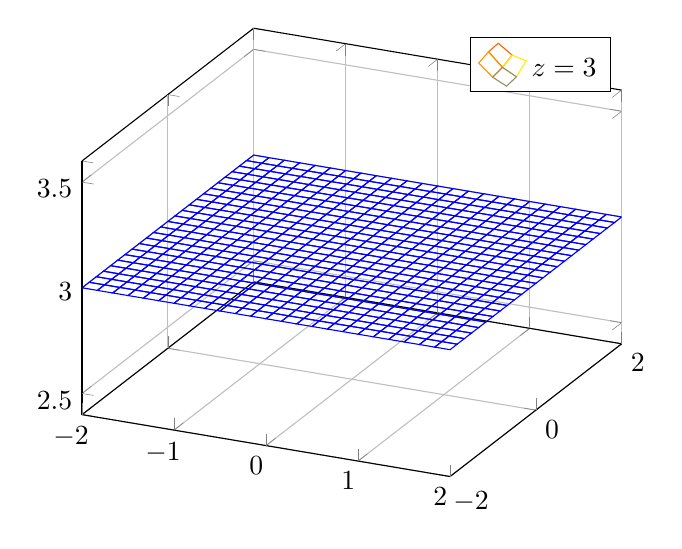
\begin{tikzpicture}
        \begin{axis}[grid=major]
          \addplot3[mesh,domain=-2:2,y domain=-2:2]{3};
          \addlegendentry{$z = 3$}
        \end{axis}
      \end{tikzpicture}
    \end{center}
    Meanwhile, $y=0$ would be a ``wall'' that passes through the origin that contains the line $y=0$ in the $xy$ plane.\\

    Finally, $z = x+y+1$ is a plane, as we can see below.
    \begin{center}
      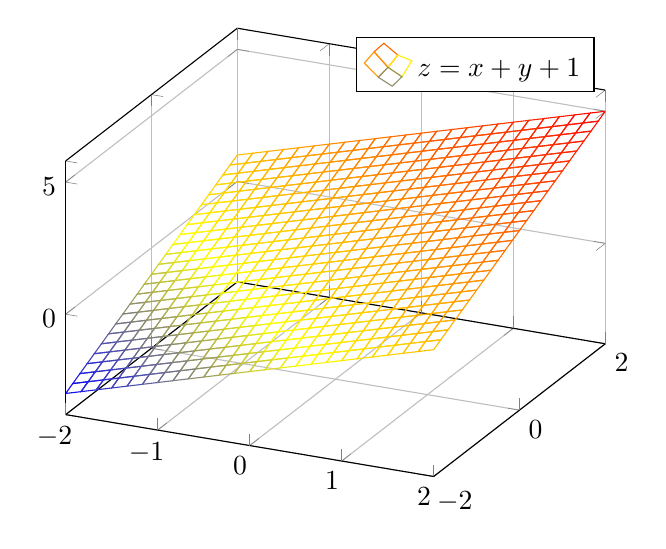
\begin{tikzpicture}
        \begin{axis}[grid=major]
          \addplot3[mesh,domain=-2:2,y domain=-2:2]{x+y+1};
          \addlegendentry{$z = x+y+1$}
        \end{axis}
      \end{tikzpicture}
    \end{center}
  \end{problem}
  \begin{problem}{Visualizing a function of multiple variables}
    Consider the function $f(x,y) = x^2-y^2$. We can try visualizing slices as follows:
    \begin{itemize}
      \item $f(-2,y) = 4-y^2$
      \item $f(0,y) = -y^2$
      \item $f(2,y) = 4-y^2$
      \item $f(x,-2) = x^2+4$
      \item $f(x,0) = x^2$
      \item $f(x,2) = x^2+4$
    \end{itemize}
    %\begin{center}
    %  \begin{tikzpicture}
    %    \begin{axis}[grid=major]
    %      \addplot3[mesh,domain=-4:4,y domain=-4:4]{x^2-y^2};
    %      \addlegendentry{$z = x+y+1$}
    %    \end{axis}
    %  \end{tikzpicture}
    %\end{center}
    Alternatively, we can visualize via contour diagrams (i.e., everywhere that $z$ is a certain value), as seen in mathematica as follows:
    \begin{tcbraster}[raster columns = 1,colframe = black!75!white,colback=white, title=Contour Diagram]
      \tcbincludepdf{images/contour_1.pdf}
    \end{tcbraster}
  \end{problem}
  \begin{problem}{Contour Example}
    Consider the function $f(x,y) = y-3x^2$. We want to find the contours.
    \tcblower
    For any $c$, we have that $c = y-3x^3$, or $y = 3x^3 + c$. Therefore, every contour ``looks like'' $3x^3 + c$ for values of $c$. For example, in the following, we have $c = \{-2,-1,0,1,2\}$ 
   \begin{tcbraster}[raster columns = 1,colframe = black!75!white,colback=white]
     \tcbincludepdf{images/contour_2.pdf}
   \end{tcbraster}
  \end{problem}
  \begin{problem}{Distance}
    In $\mathbb{R}^5$, let $p = (3,1,4,1,5)$, and $q = (1,0,-2,0,2)$. Using the Euclidean metric, we can find the distance between $p$ and $q$ is $d(p,q) = ((3-1)^2 + (1-0)^2 + (4-(-2))^2 + (1-0)^2 + (5-2)^2)^{1/2}= (4+1+36+1+9)^{1/2} = \sqrt{51} = 7.14$. We can also call this the $2$-norm.

    \[
      d(p,q) = \left(\sum_{k=1}^{n} (p_k-q_k)^2\right)^{1/2}
    \] 
  \end{problem}
  \begin{problem}{Derivatives}
    \begin{center}
      \includegraphics[width=10cm]{contour_3}
    \end{center}
    To denote a derivative, we can't talk about one value, we must use a \textit{partial} derivative, $\frac{\partial f}{\partial x}$, or $\frac{\partial f}{\partial y}$. The closeness of the contours specifies both resolution and steepness.\\

    We can estimate slope by calculating the difference between two contours, divided by the distance between them along a path.\\

    We can also analyze via a table:
    \begin{center}
      \renewcommand{\arraystretch}{1.5}
      \begin{tabular}{c|c|c|c}
        x\symbol{92}y & 0 & 1 & 2 \\
        \cline{2-4}
        4 & 5 & 6 & 7 \\
        \hline
        6 & 8 & 9 & 10 \\
        \hline
        8 & 11 & 12 & 13
      \end{tabular}
    \end{center}
    A ``linear'' approximation for a function of two variables is expressed as follows:
    \[
      z-z_0 = m(x-x_0) + n(y-y_0)
    \] 
    Where $(x_0,y_0,z_0)\in \mathbb{R}^3$, and is an output in $z=f(x,y)$, and $m,n\in \mathbb{R}$.\\

    For example, with the above table, we can see that the function is linear in $x$ and $y$ (i.e., the slope holding the other variable constant is constant).
  \end{problem}
  \begin{problem}{Limits in Multivariable Functions}
    Consider the following:
    \[
      \lim_{(x,y)\rightarrow (0,0)} \frac{x^2 + y^2}{x^2-y^2}
    \] 
    Allow $y = mx$
    \begin{align*}
      \lim_{(x,y)\rightarrow (0,0)} \frac{x^2 + y^2}{x^2-y^2}&= \lim_{(x,y)\rightarrow (0,0)} \frac{x^2 + (mx)^2}{x^2 - (mx)^2}\\
                                                             &= \frac{1+m^2}{1-m^2}
    \end{align*}
    Thus, the limit must depend on the path taken. The following table shows the limits for different values of $m$
    \begin{center}
      \begin{tabular}{c|c}
        $m$ & $\displaystyle\lim_{(x,y)\rightarrow (0,0)} \frac{x^2 + y^2}{x^2 - y^2}$\\
        \hline
        0 & $1$\\
        1 & undefined\\
        2 & $-\frac{5}{3}$
      \end{tabular}
    \end{center}
    Because the limit depends on the path of incidence, we have that the limit is \textbf{undefined}.\\

    For graphs where the contours ``approach'' a particular point, we can see that the limit is defined.
  \end{problem}
  \begin{problem}{Vectors}
    A vector is a mathematical object with direction and magnitude:
    \[
      \vec{v} = \begin{bmatrix}
        3\\1\\4
      \end{bmatrix}
    \] 
    Alternatively, we can have $\vec{w} = \begin{bmatrix}3&1&4\end{bmatrix}$. These vectors are equivalent because they are components of $\mathbb{R}^3$.\\

    Vector addition is \textit{component-wise}, (i.e., you add or subtract components in order to find the new vectors).
    \begin{problem}{Direction of $\vec{v}$}
      \[
        \frac{\vec{v}}{\Vert\vec{v}\Vert}
      \] 
    \end{problem}
    \begin{problem}{Properties of Vectors}
      Let $\vec{u},\vec{v}\in \mathbb{R}^n$. Via properties of the real numbers, we know the following:
      \begin{itemize}
        \item $\vec{u} + \vec{v} = \vec{v} + \vec{u}$
        \item $(\vec{u} + \vec{v}) + \vec{w} = \vec{u} + (\vec{v} + \vec w)$
        \item $c\vec{u} = \langle cu_1,cu_2,\dots,cu_k\rangle$
      \end{itemize}
      Additionally, we define $\vec{u} \cdot \vec{v}$ as follows:
      \[
        \vec{u} \cdot \vec{v} = \sum_{k = 1}^{n} u_kv_k = \Vert\vec{u}\Vert\Vert\vec{v}\Vert\cos\theta
      \] 
    \end{problem}
  \end{problem}
  \begin{problem}{Partial Derivatives}
    Consider $f(x,y) = x^2y + xe^y$.
    \begin{align*}
      f_x &:= \frac{\partial f}{\partial x}\\
      f_x(a,b) &= \frac{\partial f}{\partial x}\biggr\rvert_{(a,b)}
    \end{align*}
    We know that $f\in C^{\infty}(\mathbb{R} \times \mathbb{R})$, meaning $f$ is endlessly differentiable.
  \end{problem}
  \begin{problem}{Functions and Approximations}
    Let $f(x,y) = x^2 - y^2$, $g(x,y) = 2xy$
    \begin{itemize}
      \item $f_{xx} + f_{yy} = 0$
      \item $g_{xx} + g_{yy} = 0$
    \end{itemize}
    This is the solution to the Laplace equation:
    \begin{align*}
      0 &= \frac{\partial^2 f}{\partial x^2} + \frac{\partial^2 f}{\partial y^2}
    \end{align*}
    For $f(x,y)$ at $(a,b,f(a,b))$, we have the following:
    \begin{align*}
      \ell(x,y) &= f(a,b) + f_x(a,b)(x-a) + f_y(y-b)\\
      q(x,y) &= \ell(x,y) + \frac{1}{2}\left(f_{xx}(a,b)(x-a)^2 + 2f_{xy}(a,b)(x-a)(y-b) + f_{yy}(a,b)(y-b)^2\right)\\
    \end{align*}
    In order to get a sense of the ``derivative,'' we can use the following:
    \begin{align*}
      \nabla f(x,y) = \langle f_x(x,y),f_y(x,y)\rangle
    \end{align*}
  \end{problem}
  \begin{problem}{Directional Derivative and Gradient}
    Given $f(x,y)$ and $(a,b)$, where $f\in C^{2}(\mathbb{R}^2)$. Then, the quadratic approximation is:
    \begin{align*}
      f(x,y) &\approx f(a,b) + f_{x}(a,b)(x-a) + f_x(a,b)(y-b)\\
             &+ \frac{1}{2}\left(f_{xx}(a,b)(x-a)^2 + f_{yy}(a,b)(y-b)^2 + f_{xy}(a,b)(x-a)(y-b)\right)\\
          df &= f_x(a,b)dx + f)y(a,b)dy \tag*{a differential}\\
      \Delta f &= f_x(a,b)\Delta x + f_y(a,b)\Delta y\\
      \shortintertext{Evaluating $f(x,y) = xe^y$ at $(a,b) = (-1,0)$}
      f_x &= e^y\\
      f_y &= xe^y\\
      f_x(-1,0) &= 1\\
      f_y(-1,0) &= -1\\
      \Delta f &= \Delta x - \Delta u
    \end{align*}
    On a given contour map, let $\vec u = \langle u_1,u_2\rangle$ denote a \textit{unit} vector in a direction that we want to find the derivative of $f$ in.
    \begin{align*}
      f_{\vec u}(x,y) &= \nabla f(a,b) \cdot \vec u\\
      \shortintertext{Where}
      \nabla f(a,b) &= \langle f_x(a,b),f_y(a,b)\rangle
    \end{align*}
  \end{problem}
\end{document}
